\documentclass{article}
\usepackage{amsmath,amsthm,amssymb}
\usepackage {mathtext}
\usepackage{amsfonts} 
\usepackage[T1,T2A]{fontenc}
\usepackage[utf8]{inputenc}
\usepackage [english, russian] {babel}
\usepackage[babel=true]{microtype}
\usepackage{caption}
\usepackage{subcaption}
\captionsetup[table]{position=t,justification=raggedleft,slc=off}
\setlength{\abovecaptionskip}{0pt}
\usepackage {geometry}
\usepackage{graphicx}
\usepackage{multirow}
\geometry{margin=2cm}
\title{Лабораторная работа №1.3.1 \\ Определение модуля Юнга на основе исследования деформаций растяжения и изгиба}
\author{Павел Рудачихин \\ группа Б04-507}
\date{16.10.2025}
\begin {document}
\maketitle

\section* {Аннотация} 

\hspace{4mm} В работе определяется модуль Юнга и проверяется закон Гука. Исследуются погрешности проводимых измерений.

\textbf{Цель работы:} экспериментально получить зависимость между напряжением и деформацией - закон Гука - для двух простейших напряжённых состояний упругих тел: одноосного растяжения и чистого изгиба; по результатам измерений вычислить модуль Юнга.

\textbf{В первой части работы используются:} прибор Лермантова, проволока исследуемого материала, лазерный указатель, шкала, набор грузов, рулетка, весы.

\textbf{Во второй части работы используются:} стойка для изгибания балки, индикатор величины прогиба, набор балок, набор грузов, линейка, штангенциркуль, весы.

\textbf{Методы:} 1) определение  углового  коэффициента  наклона  зависимости двух величин; 2) измерение геометрических размеров с помощью штангенциркуля и микрометра; 3) измерение массы тел с помощью весов; 4) измерение расстояния с помощью рулетки; 5) измерение изменения положения точки лазерного указателя с помощью линейки-шкалы; 6) измерение величин прогиба с помощью стрелочного индикатора. 


\section* {Теоретические сведения}
\subsection* {Модули упругости}

\hspace{4mm} \textit{Деформация} в точке по определению равна $\varepsilon = \dfrac{ds}{dx} $, т.е. деформация - это относительное смещение двух точек, делённое на первоначальное расстояние между ними. Напряжение - сила, отнесённая к единице площади: $\sigma = \dfrac{F}{S} $

Если направление $ds$ совпадает с направлением $dx$, то имеет место деформация \textit{растяжения (сжатия)}. Если $ds$ перпендикулярен $dx$, то имеет место деформация \textit{сдвига} (см. рис. 1).

\begin{figure}[h!]
	\centering
	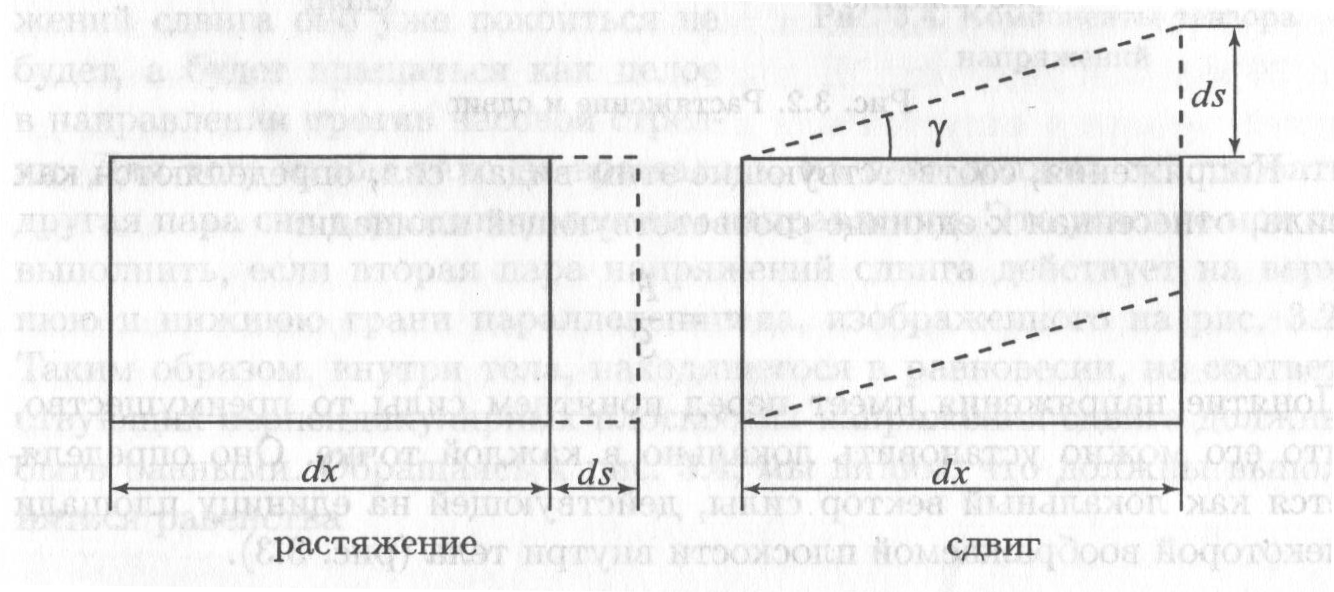
\includegraphics[width=0.5\linewidth]{1}
	\caption{Основные виды деформаций}
	\label{fig:1}
\end{figure}


На основе эмпирических данных получены следующие соотношения для растяжения и для сдвига соответственно:

\begin{equation} 
	\sigma = E\varepsilon, \ \ \sigma = G\varepsilon,
\end{equation}

где $E$ - \textit{модуль Юнга}, a $G$ -\textit{ модуль сдвига}.

Данные соотношения являются формой записи \textbf{закона Гука}, который справедлив для \textit{упругих} деформаций - устраняющихся при снятии внешней силы, вызвавшей деформации. Линейная зависимость сохраняется на интервале от нуля до некоторой предельной деформации. Далее имеет место \textit{необратимая}, или \textit{пластическая}, деформация, зависимость которой от напряжения имеет нелинейный характер (см. рис. 2).



\begin{figure}[h!]
	\centering
	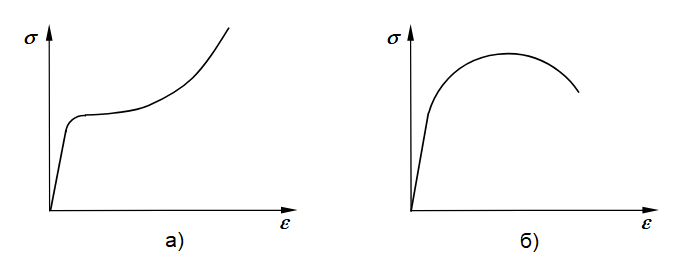
\includegraphics[width=0.5\linewidth]{2}
	\caption{а) график сжатия пластичного материала; б) график сжатия хрупкого материала.}
	\label{fig:2}
\end{figure}

\section* {Методика измерений}
\subsection* {Прибор Лермантова}

\hspace{4mm} Удлинение проволоки можно определить экспериментально с помощью \textit{прибора Лермантова}. Схема установки представлена на рисунке 3а.

\begin{figure}[h!]
	\centering
	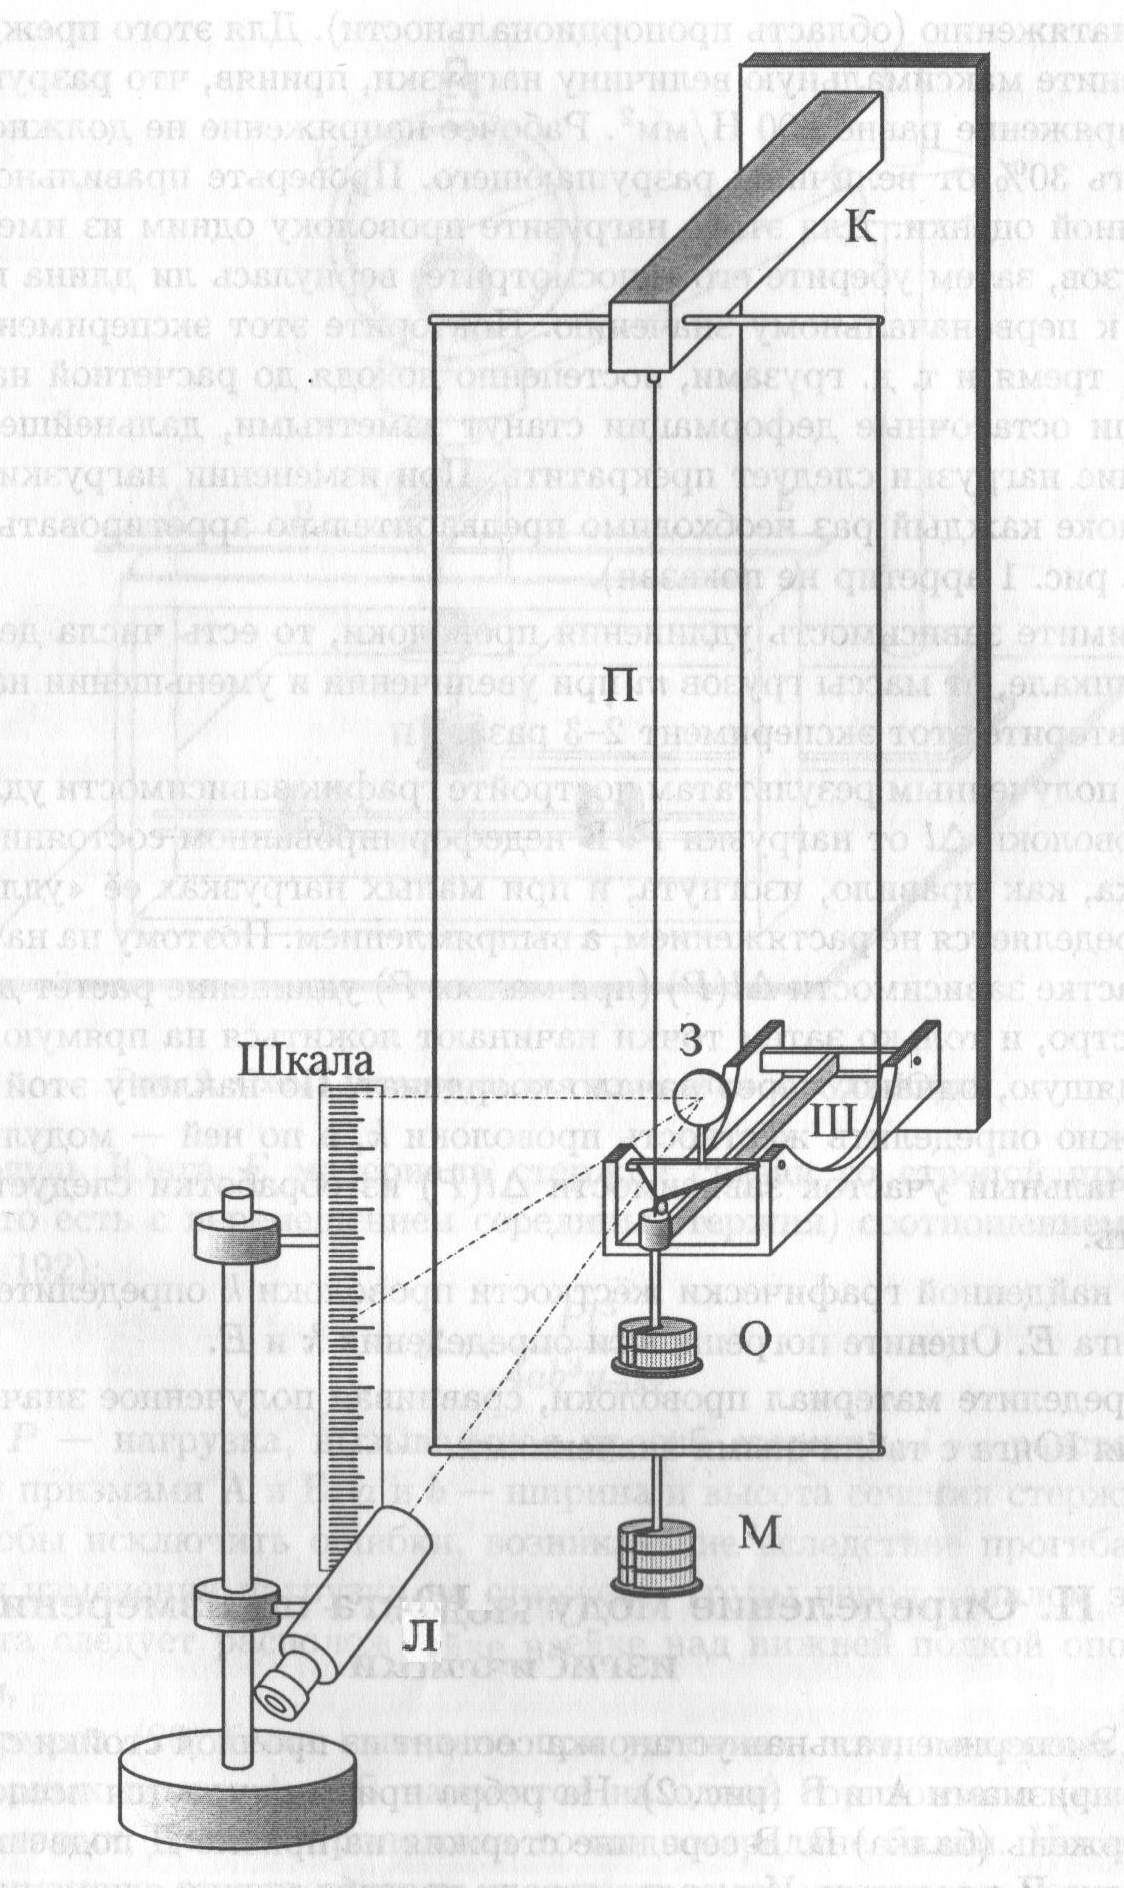
\includegraphics[width=0.3\linewidth]{3}
	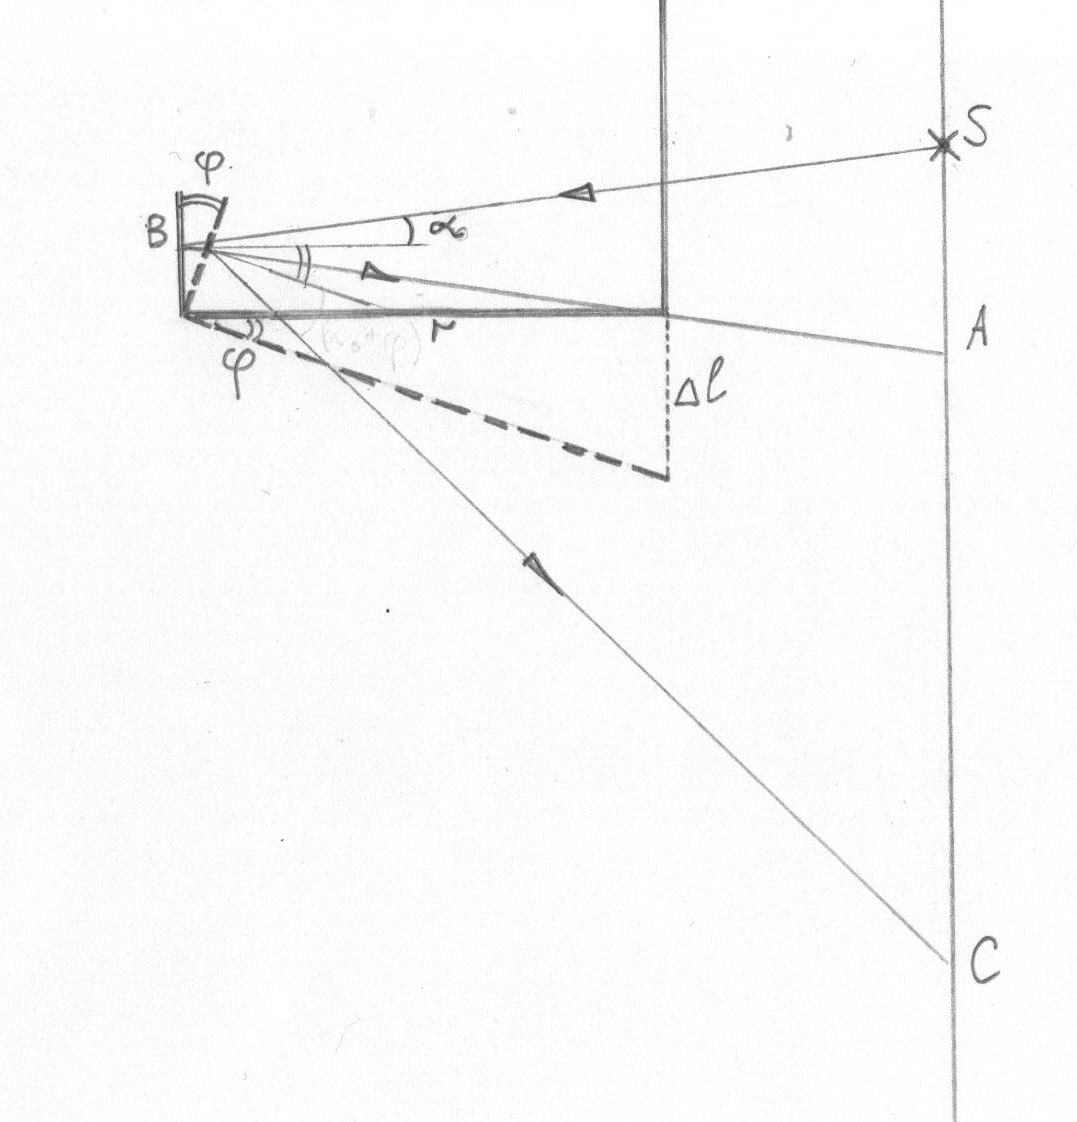
\includegraphics[width=0.4\linewidth]{4}
	\caption{
		\small а) Прибор Лермантова: К - кронштейн, П - проволока, З - зеркало, Ш - шарнирный кронштейн, О - площадка для огрузки, М - площадка для хранения грузов, Л - лазерный указатель.
		б) К выводу формулы 3: S - лазерный указатель, В - точка отражения луча, Н - основание перпендикуляра из В к шкале, т.е. ВН = h - расстояние от зеркала до шкалы, А - начальное положение лазерной метки, С - конечное положение лазерной метки; $\alpha$ - угол между лучом и перпендикуляром, $\varphi$ - угол поворота рычага, $\Delta l$ - удлинение проволоки, $r$ - длина рычага.}

\end{figure}


В этом приборе нижний конец проволоки связан с рычагом, на котором расположено зеркало. Угол поворота зеркала зависит от удлинения проволоки, а угол можно определить по перемещению метки отражённого лазерного луча по шкале-линейке (см. рис. 3б).



Угол $\varphi$ и высота зеркала малы. Поэтому перемещением точки отражения В можно пренебречь. $\angle HBC = \alpha + 2\varphi$ , $\angle HBA = \alpha + 2\varphi$, $HA = h tg\alpha$, $HC = h tg(\alpha+2\varphi)$. Так как углы малы, положим значения тангенса равными радианной мере углов: $HA = h\alpha$, $HC = h (\alpha+2\varphi)$. Тогда $AC = HC-HA = 2h\varphi$. По тем же приближениям $\varphi = \Delta l / r$. Пусть $AC = b$. Имеем формулу связи измеряемого смещения метки с удлинением проволоки:

\begin{equation}
	\Delta l = \dfrac{b r}{2 h}
\end{equation}

\subsection* {Установка для изгибания балки}

\hspace{4mm} Прогиб балки можно определить экспериментально с помощью установки, изображённой на рис. 4.

\begin{figure}[h!]
	\centering
	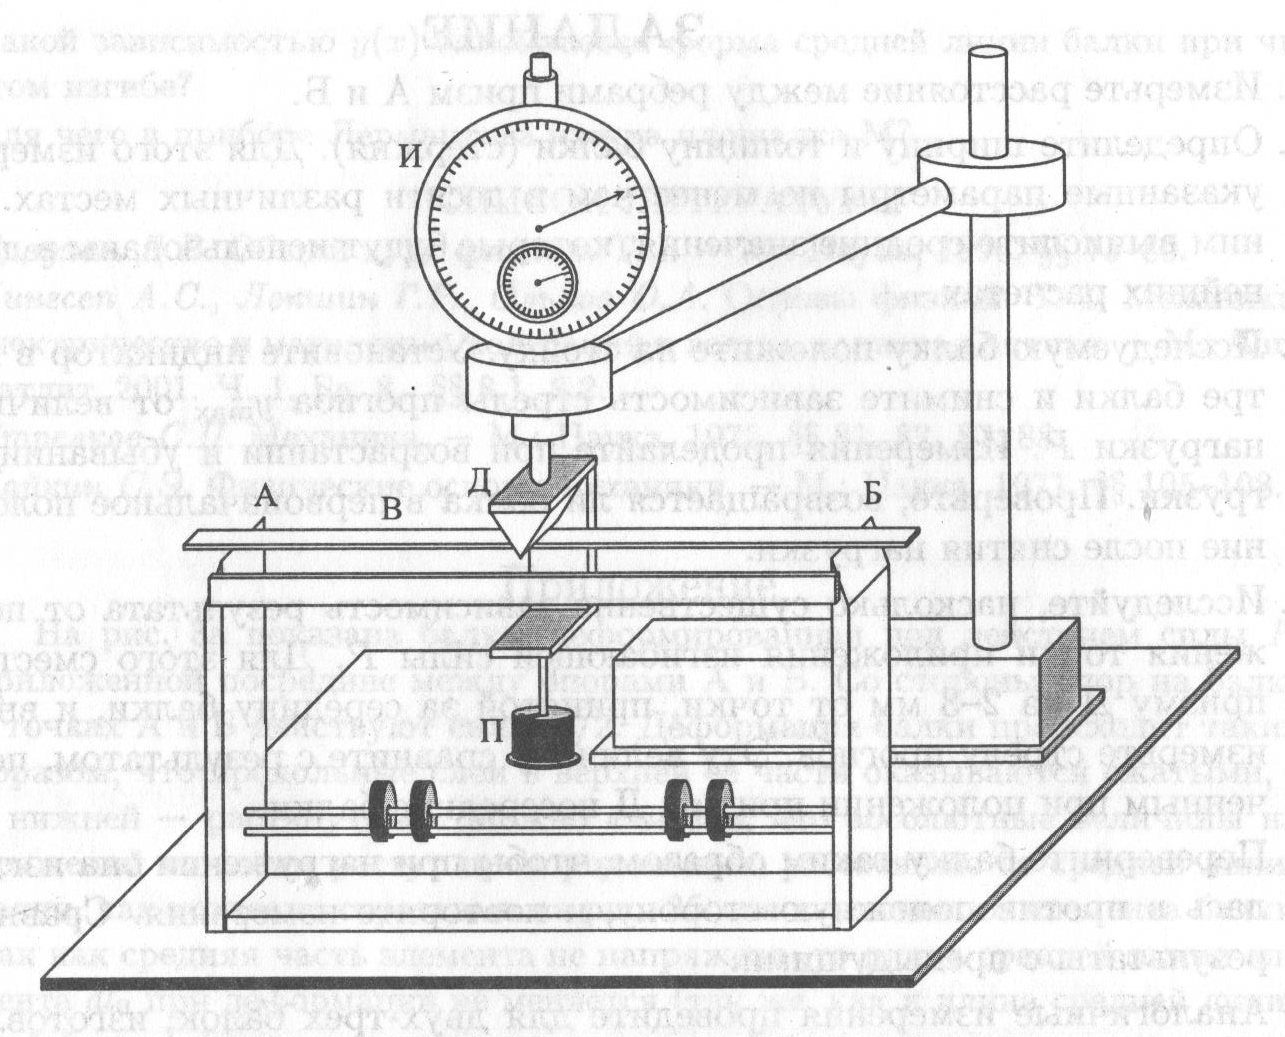
\includegraphics[width=0.6\linewidth]{5}
	\caption{Установка для изгибания балки: И - индикатор, А и Б - опорные призмы, Д - нагрузочная призма, В - исследуемый стержень (балка), П - площадка с грузами.}
	\label{fig:5}
\end{figure}


Исследуемый стержень опирается на рёбра призм А и Б. В середине стержня на призме Д подвешена площадка П с грузами. Прогиб стержня в этом месте измеряется стрелочным индикатором И.

На данной установке можно определить модуль Юнга по следующей формуле:

\begin{equation}
	E = \dfrac{P l^{3}}{4 a b^{3} y},
\end{equation}

где $P$ - вес груза, $l$ - расстояние между опорными призмами, $a$ - ширина балки, $b$ - её высота, $y$ - перемещение середины стержня (стрела прогиба).

\section*{Используемое оборудование}

\hspace{4mm} В данной работе для измерения массы использованы цифровые \textbf{весы}. Погрешность измерения массы определена как три в последнем разряде дисплея прибора: $\Delta_{\text{m}} = \pm 0,3$ г

Погрешность \textbf{линейки-шкалы} составляет $\Delta_{\text{Л}} = \pm 0,5$ мм 

Погрешность \textbf{большой линейки} составляет $\Delta_{\text{БЛ}} = \pm 2$ мм

Погрешность \textbf{штангенциркуля} определена маркировкой производителя: $\Delta_{\text{Ш}} = \pm 0,1$ мм

Погрешность \textbf{микрометра} определена маркировкой производителя: $\Delta_{\text{М}} = \pm 0,01$ мм

Погрешность \textbf{индикатора} определена ценой деления: $\Delta_{\text{И}} = \pm 0,01$ мм

Погрешность \textbf{рулетки} определена ценой деления: $\Delta_{\text{Р}} = \pm 1$ мм


\section*{Результаты измерений}

\subsection*{Параметры установок}

Параметры прибора Лермантова приведены в таблице 1.  

\begin{table}[h!]
	\centering
	\captionbox{Параметры прибора Лермантова}{
		\begin{tabular}{|c|c|}
			\hline
			Параметр  & Значение  \\
			\hline
			Длина проволоки, $l$ & $(1760 \pm 2)$ мм \\
			\hline
			Длина рычага, $r$  & $(13 \pm 1)$ мм  \\
			\hline
			Диаметр проволоки, $d$  & $(0,73 \pm 0,01)$ мм \\
			\hline
			Расстояние от зеркала до шкалы, $h$  & $(1476 \pm 1)$ мм \\
			\hline
			
	\end{tabular}}
\end{table}

Расстояние между опорными призмами установки изгибания балки составляет $(500,0 \pm 0,5)$ мм.

\subsection*{Первая часть} 

По известному диаметру проволоки определена площадь её поперечного сечения:

\begin{equation}
	S = \frac{\pi d^{2}}{4} \approx 0.418 \ {мм}^{2} ; \ \sigma_S = S \cdot \varepsilon_S = S  \cdot 2 \varepsilon_d \approx 0.011 \ {мм}^{2}
\end{equation}

В начале первой части работы определены границы области упругой деформации. Сначала произведена оценка: рабочее напряжение принято за 30 \% от разрушающего, равного $ \hat{\sigma} = 900 \ Н/мм^{2}$. Далее оценена максимальная масса грузов:

\begin{equation}
	\hat{m} = \frac{\hat{P}}{g} = \frac{0,3\cdot \hat{\sigma} \cdot S}{g} \approx 11,5 \ кг
\end{equation}

На практике лазерная метка перестала возвращаться в исходное положение уже при подвешивании 8 грузов, т.е. при 2,7 кг.

Зависимость положения лазерного указателя на шкале от массы грузов представлена в таблице 2.

\begin{table}[h!]
	\centering
	\captionbox{Зависимость положения метки от массы груза}{
	\begin{tabular}{|r|r||r|r|}
		\hline
		$m$, кг&     $x$, мм     &    $m$, кг      &  $x$, мм \\
		\hline
		0,0       & 198      & 0,0        & 198 \\
		\hline
		245,6    & 239      & 478,3    & 226 \\
		\hline
		491,0      & 256      & 724,0      & 244 \\
		\hline
		736,5    & 269      & 969,4    & 257 \\
		\hline
		981,9    & 282      & 1214,9   & 272 \\
		\hline
		1227,6   & 293      & 1460,3   & 285 \\
		\hline
		1705,9   & 307      & 1705,9   & 308 \\
		\hline
		1227,6   & 294      & 1460,3   & 285 \\
		\hline
		981,9    & 281      & 1214,9   & 272 \\
		\hline
		736,5    & 269      & 969,4    & 258 \\
		\hline
		491 ,0     & 256      & 724,0    & 244 \\
		\hline
		245,6    & 241      & 478,3    & 228 \\
		\hline
		0,0      & 198      & 0,0        & 199 \\
		\hline
	\end{tabular}}
\end{table}

\subsection*{Вторая часть} 

Сначала измерены геометрические размеры образцов - латунного и деревянного брусков (см. табл. 3-4).

\begin{table}[h!]
	\centering
	\captionbox{Геометрические размеры латунного бруска}{
	\begin{tabular}{|r|r|r|r|r|r|r|r|r|r|r|}
		\hline
		Высота, мм & 3,9      & 3,9      & 3,9      & 3,9      & 3,9      & 3,9      & 3,9      & 3,9      & 3,9      & 3,9 \\
		\hline
		Ширина, мм & 21,1     & 21,2     & 21,2     & 21,2     & 21,4     & 21,5     & 21,4     & 21,4     & 21,4     & 21,3 \\
		\hline
	\end{tabular}}
\end{table}

\begin{table}[h!]
	\centering
	\captionbox{Геометрические размеры деревянного бруска}{
	\begin{tabular}{|r|r|r|r|r|r|r|r|r|r|r|}
		\hline
		Высота, мм & 9,9      & 9,9      & 9,8      & 9,9      & 9,9      & 10,0       & 10,0       & 9,9      & 9,9      & 9,8 \\
		\hline
		Ширина, мм  & 20,4     & 20,2     & 20,3     & 20,6     & 20,4     & 20,4     & 20,3     & 20,3     & 20,2     & 20,0 \\
		\hline
	\end{tabular}}
\end{table}

Затем снята зависимость стрелы прогиба от массы груза при возрастании и убывании нагрузки. Образцы нагружены с двух противоположных сторон. Измерения представлены в таблице 5.

\begin{table}[h!]
	\centering
	\captionbox{Зависимость стрелы прогиба $y$ от массы груза, где $y_1$ - на одной стороне, $y_2$ - на другой}{
	\begin{tabular}{|r|r|r|r|r|}
		\hline
		\multicolumn{1}{|c|}{\multirow{2}[4]{*}{Масса, г}} & \multicolumn{2}{c|}{Латунь} & \multicolumn{2}{c|}{Дерево} \\
		\cline{2-5}             & \multicolumn{1}{c|}{$y_1, 10^{-2}$  мм} & \multicolumn{1}{c|}{$y_2, 10^{-2}$ мм} & \multicolumn{1}{c|}{$y_1, 10^{-2}$ мм} & \multicolumn{1}{c|}{$y_2, 10^{-2}$ мм} \\
		\hline
		501,0    & 120      & 123      & 75       & 75 \\
		\hline
		1008,0   & 250      & 245      & 150      & 150 \\
		\hline
		1504,8   & 364      & 365      & 228      & 226 \\
		\hline
		1959,3   & 484      & 484      & 298      & 298 \\
		\hline
		2456,2   & 594      & 595      & 370      & 373 \\
		\hline
		2912,5   & 695      & 704      & 444      & 446 \\
		\hline
		3386,0   & 834      & 815      & 545      & 535 \\
		\hline
		2912,5   & 725      & 710      & 450      & 453 \\
		\hline
		2456,2   & 615      & 590      & 380      & 381 \\
		\hline
		1959,3   & 499      & 490      & 305      & 307 \\
		\hline
		1504,8   & 381      & 380      & 235      & 236 \\
		\hline
		1008,0   & 255      & 253      & 138      & 160 \\
		\hline
		501,0    & 124      & 128      & 80       & 80 \\
		\hline
	\end{tabular}}

\end{table}


\section*{Обработка результатов}

\hspace{4mm} Все вычисления произведены с использованием программы, написанной специально для этих целей на языке программирования Python. Построение графиков выполнено с помощью модуля Matplotlib. Исходный код программы содержится в электронном приложении к работе.

\subsection*{Первая часть}
 
\begin{figure}[h!]
	\centering
	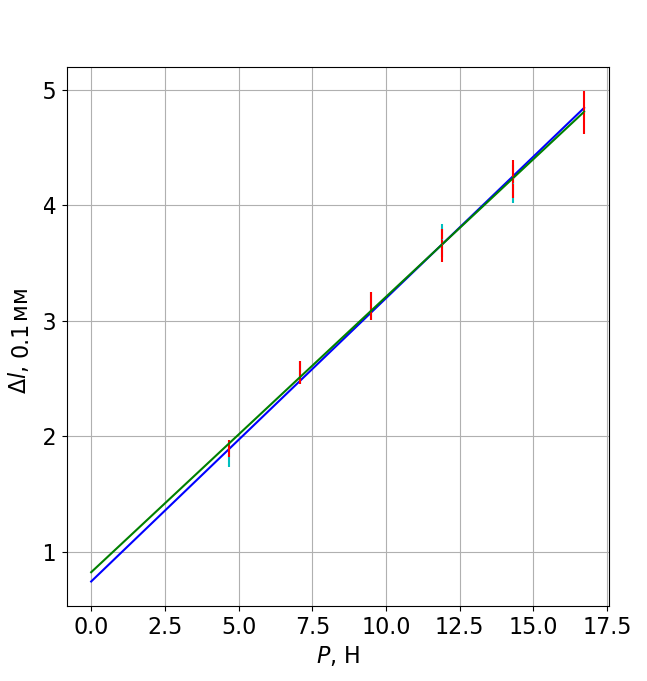
\includegraphics[width=0.5\linewidth]{plot1}
	\caption{Зависимость удлинения проволоки от веса при убывании и возрастании нагрузки}
\end{figure}

\begin{figure}[h!]
	\centering
	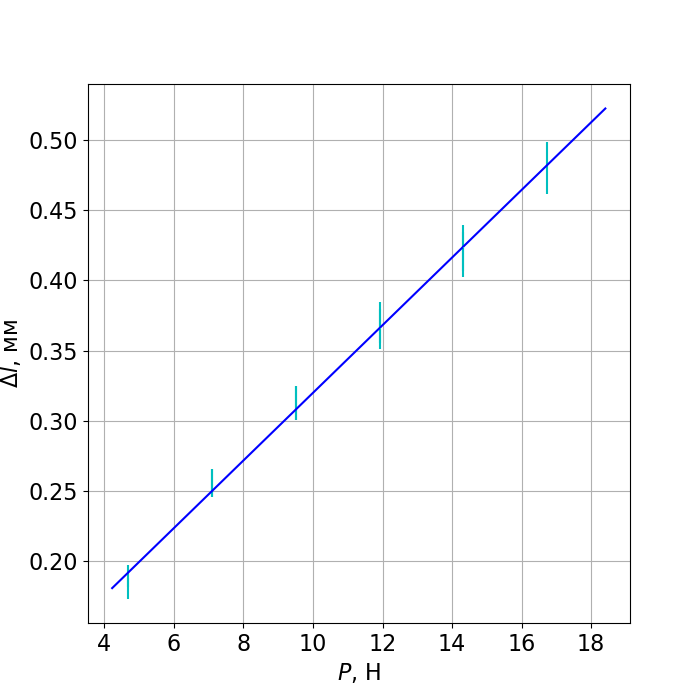
\includegraphics[width=0.45\linewidth]{plot11}
	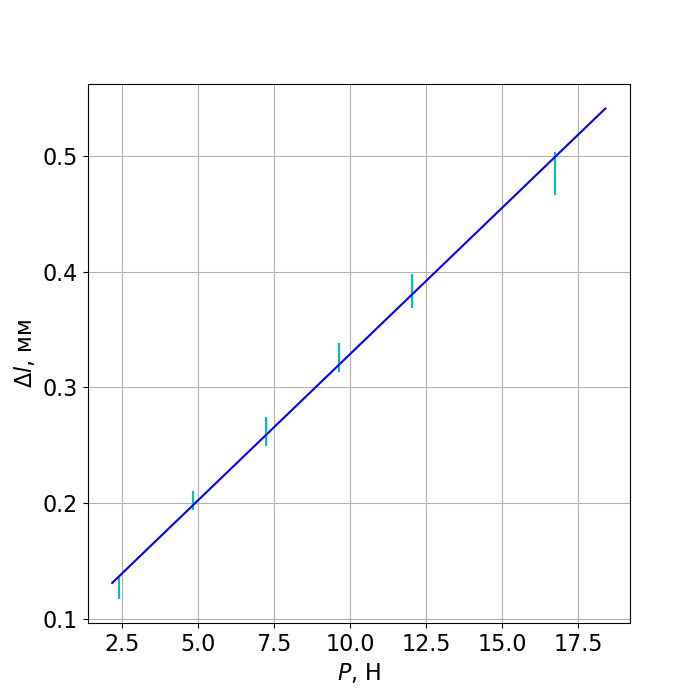
\includegraphics[width=0.45\linewidth]{plot12}
	\caption{График зависимости удлинения проволоки от веса нагрузки}
\end{figure}

\hspace{4mm} Определено, что коэффициент жёсткости при возрастании и убывании нагрузки меняется незначительно, в пределах погрешности измерений (см. рис. 5). По методу наименьших квадратов вычислены угловые коэффициенты и их случайные погрешности в двух опытах. В соответствии с этим проведены прямые на графике по экспериментальным точкам (см. рис. 6). По полученным значениям угловых коэффициентов прямой $k$ и параметрам установки вычислен модуль Юнга: 

\begin{equation}
	E = \frac{l}{S k}
\end{equation}

Заметим, что погрешность измерения массы грузов возрастает при добавлении грузов, т.к. итоговая масса есть сумма измеренных масс. Погрешность суммы определена по формуле:

\begin{equation}
	\sigma_{m_1 + m_2} = \sqrt{\sigma_{m_1}^{2} + \sigma_{m_2}^{2}}
\end{equation}

Относительная систематическая погрешность коэффициента вычислена по формуле:

\begin{equation}
	\varepsilon_{k} = \sqrt{\varepsilon_{P}^2 + \varepsilon_{\Delta l}^2} =  \sqrt{\varepsilon_m^2 + \varepsilon_b^2 + \varepsilon_r^2 + \varepsilon_h^2}
\end{equation}

Полная погрешность коэффициента определена так:

\begin{equation}
	\sigma_{полн} = \sqrt{\sigma_{случ}^{2}+\sigma_{сист}^{2}}
\end{equation}

Относительная погрешность модуля Юнга вычислена по формуле:

\begin{equation}
	\varepsilon_{G} = \sqrt{\varepsilon_l^2 + \varepsilon_S^2 + \varepsilon_k^2}
\end{equation}

В результате получаем:

\begin{equation}
	\boxed{k_1 = (22,9 \pm 0,9) \ кН/м; \ \ k_2 = (22,3 \pm 0,9) \ кН/м}
\end{equation}


\begin{equation}
	\boxed{E_1 = (184 \pm 9) \ ГПа; \ \ E_2 = (188 \pm 9) \ ГПа}
\end{equation}

Полученные значения модуля Юнга с учётом погрешности соответствуют железу, (возможно, его сплавам), для которого характерны значения 190-200 ГПа.

\subsection*{Вторая часть} 

\hspace{4mm} Методы вычисления погрешностей аналогичны первой части работы. 

Зависимость "нагрузка-прогиб" имеет линейный характер. Прямая на графике (см. рис. 5) проведена по методу наименьших квадратов.

\begin{figure}[h!]
	\centering
	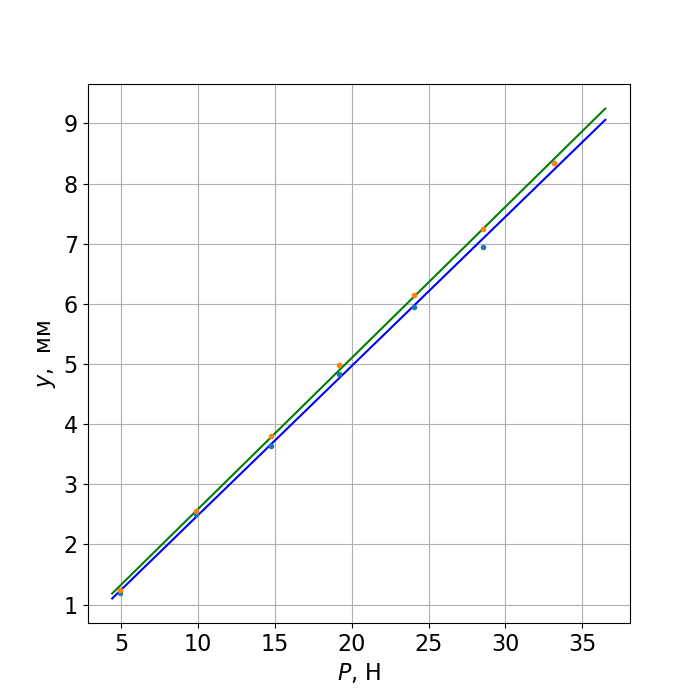
\includegraphics[width=0.45\linewidth]{plot2.1}
	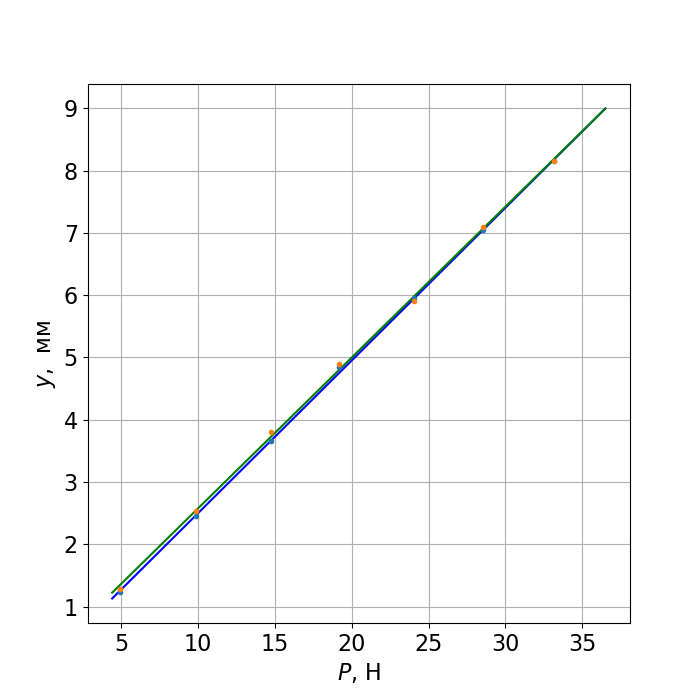
\includegraphics[width=0.45\linewidth]{plot2.2}
	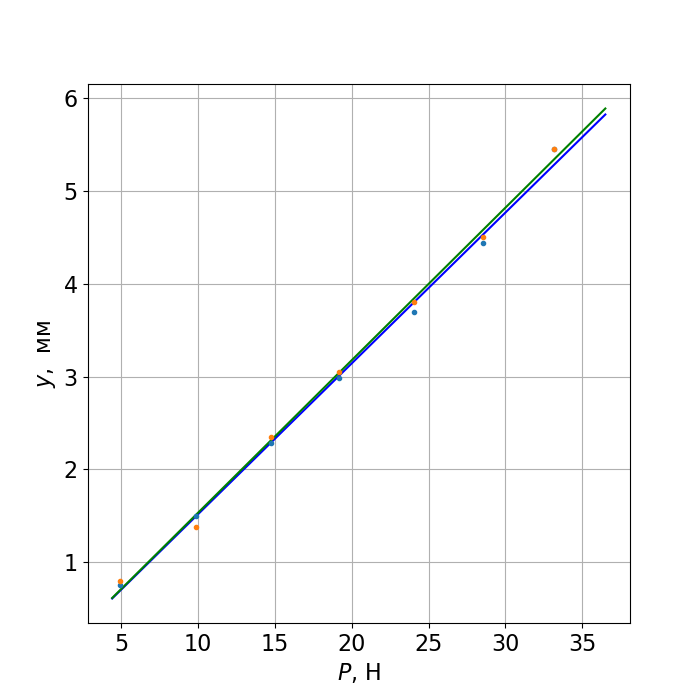
\includegraphics[width=0.45\linewidth]{plot2.3}
	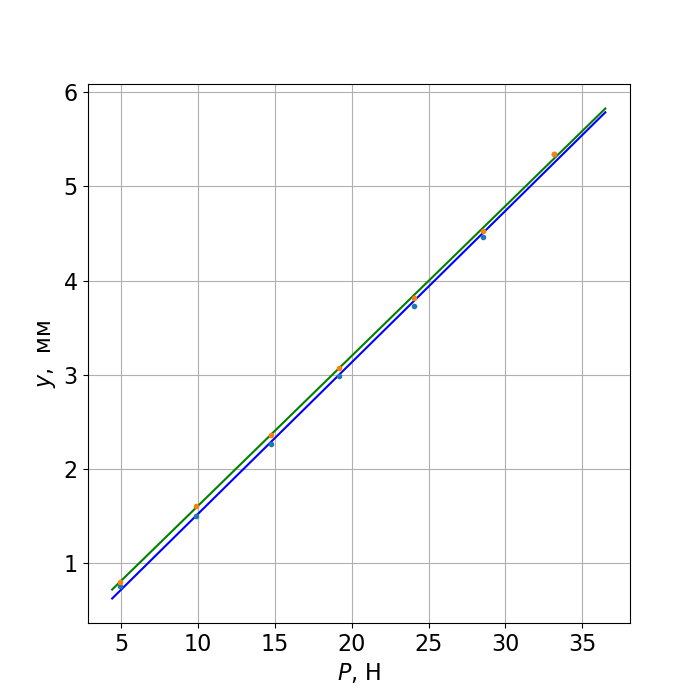
\includegraphics[width=0.45\linewidth]{plot2.4}
	\caption{Графики зависимости "нагрузка-прогиб". Слева направо и сверху вниз: латунь - лицевая сторона, латунь - оборотная сторона, дерево - лицевая, дерево - оборотная.}
\end{figure}
 

Определено, что угловой коэффициент можно считать неизменным в пределах погрешности при возрастании и убывании нагрузки, при переворачивании образца, при малом смещении точки приложения изгибающей силы от середины стержня.

\begin{figure}[h!]
	\centering
	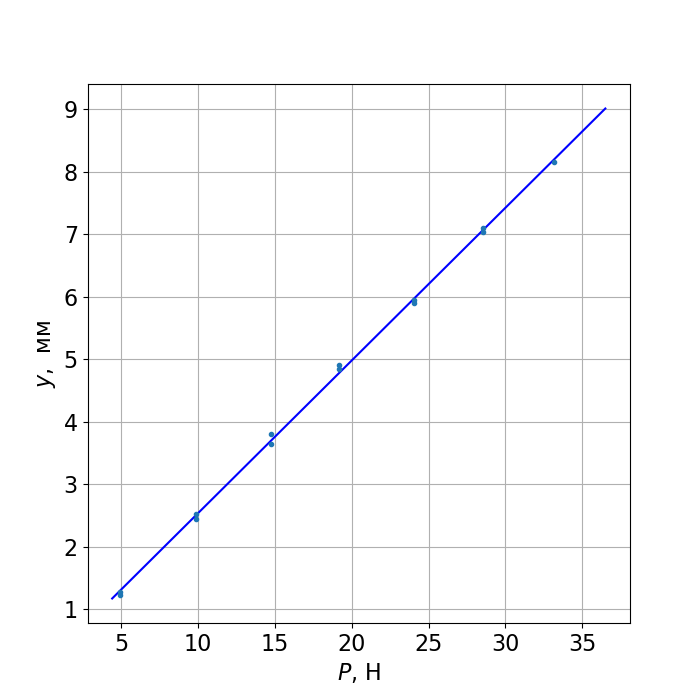
\includegraphics[width=0.45\linewidth]{plot22}
	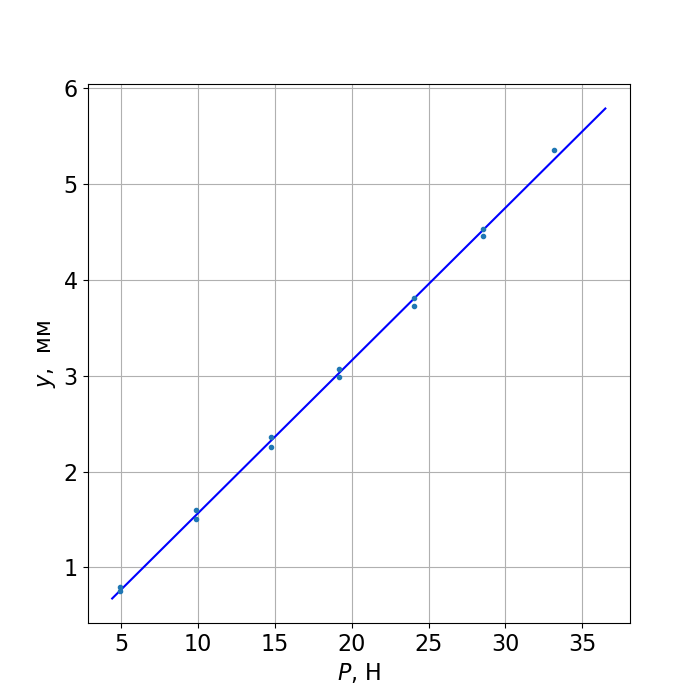
\includegraphics[width=0.45\linewidth]{plot222}

	\caption{Итоговые графики зависимости "нагрузка-прогиб" для латуни и дерева.}
\end{figure}

Вычислив модуль Юнга по формуле 3, имеем:

\begin{equation}
	\boxed{E_1 = (100 \pm 8) \ ГПа; \ \ E_2 = (9,9 \pm 0,3) \ ГПа}
\end{equation}

Полученные значения с высокой точностью соответствуют справочным данным: для латуни $E = (97 ... 102) \ ГПа$, для дерева $E = (13 ... 9) \ ГПа$.


\section*{Заключение}
\hspace{4mm} Цели работы достигнуты: экспериментально получена линейная зависимость между напряжением и деформацией для двух простейших напряжённых состояний упругих тел: одноосного растяжения и чистого изгиба, что подтверждает закон Гука; по результатам измерений вычислены модули Юнга. Они с хорошей точностью совпадают с указанными в справочных данных. 

\end {document}